% !TEX root = ../thesis-example.tex
%
\chapter{Interface sensible / hardware}
\label{ch:interfaces}

\cleanchapterquote{Komponieren heißt: über die Mittel nachdenken.\\
Komponieren heißt: ein Instrument bauen.\\
Komponieren heißt: nicht sich gehen, sondern sich kommen lassen.\\
.}{Helmut Lachenmann}{1986}

\cleanchapterquote{Fingers are not to be despised: they are great inspirers, and, in contact with a musical instrument, often give birth to subconscious ideas which might otherwise never come to life.}{Igor Stravinsky}{1936}

\vspace{-1em}
\begin{itemize}[noitemsep]
\item Faire évoluer une interface en la raffinant (De Laubier, VG).
\item Faire évoluer une interface en rajoutant des choses (Patricia Dallio)
\item Faire évoluer en supprimant des choses (Dumaux)
\item Partir de l'objet (Patrick Saint Denis)
\end{itemize}

%--------------------------------------------------------------
\section{Interface gestuelle ou interface sensible?}
Il est souvent question ``d'interface gestuelle'' lorsqu'on pense aux \glspl{IHM} utilisées pour l'interaction musicale. Comme nous l'avons vu au chapitre précédant, le geste occupe une part importante de l'interaction musicale mais les interfaces de jeu ne se restreignent pas nécessairement à la captation du geste : elle peuvent être sensible à la température, la lumière\footnote{Voir par exemple les œuvres \textit{Light Thing} de Leaf Cutter John (\url{https://youtu.be/2jIlLHfSEfs}), ou encore \textit{Light Music} de Thierry de Mey}, à la couleur, et réagir de manière générale à différentes conditions environnementales.

Par ailleurs, le geste possède un certain nombre de qualités qui ne sont pas forcément captées par l'interface, alors qu'elle sont effectivement vues et ressenties par le musicien et par le public, et contribuent ainsi à la performance.

Enfin, le "geste" qui vient contrôler les processus sonores dans les DMIs peut être de nature virtuelle, prendre la forme de motifs pré-enregistrés qui peuvent être issus de toute sorte de source de données interprétées en tant que flux temporels, tels que peut-être le cas dans la sonification de données ou l'utilisation de modèles intermédiaire. Cet aspect là sera décrit plus en détail dans le chapitre \ref{ch:algorithms}.

Il semble ainsi préférable de parler d'\textit{interface sensible}, plutôt que d'\textit{interface gestuelle} pour décrire les dispositifs d'interaction numériques pour la musique, leur caractéristique commune étant l'usage de capteurs (\textit{sensors}).

\iquote{One has to think of overall systems to get a musically useful thing-you can’t really develop a sensor without relating it to the programs that you’re going to use it with}, Max Mathews, cité dans  Chadabe 1997, p. 230)


%%%%%%%%%%%%%%%%%%%%%%%%%%%%%%%%%%%%%%%%%
\section{Interface pour composer/interpréter/improviser en live}
Articulation entre grandes formes et immédiateté : la gestion du temps de l’interaction à différentes échelles.
La performance musicale avec un DMI permet d’articuler une partie compositionnelle (échelle de temps longue) et une partie interprétation/improvisation (immédiateté de l’instant). 
Quelle design d’interface permet de répondre à l’articulation de ces 2 pôles ?

\section{La part acoustique (de l'interface des \glspl{DMI})}
Rappelons tout d'abord que les \glspl{DMI}, s'ils se caractérisent par l'usage de la computation numérique, sont aussi nécessairement des instruments électroniques, électriques et acoustiques. 
Dans le cas le plus trivial, leur acoustique se limite à la membrane du haut-parleur qui transforme \textit{in fine} le signal audio-numérique en son acoustique\footnote{Le choix des haut-parleurs peut jouer un rôle primordial, comme c'est le cas dans la musique acousmatique diffusée sur orchestre de haut-parleur ou ``acousmonium''. Voir en particulier \cite{mooney_sound_2006}}. Notons qu'à la différence des instruments acoustiques, la diffusion et la projection du son est séparée de l'interface gestuelle et, bien souvent, distante du musicien quand elle est ``spatialisée''.

La dimension acoustique peut également exister en entrée de l'instrument, au niveau son interface. L'usage de microphones, notamment de capsule piezo dites ``microphone de contact'', vient redonner une composante acoustique au corps sinon purement structurel de l'agencement instrumental.

Cette part acoustique a une place particulière en tant qu'elle affecte 



%%%%%%%%%%%%%%%%%%%%%%%%%%%%%%%%%%%%%%%%%
\section{Qualité ergodynamiques}


\subsection{Proprioception}
La proprioception désigne la perception de la position des différentes parties du corps dans l'espace, recouvrant le sens du mouvement (\textit{kinesthésie}) et le sens de la posture (\textit{statesthésie}).


%------------------------------------------------------------
\subsection{Ergodynamisme}
cf. définition de Thor Magnusson
agencement de l’interface, représentation visuelle, repères tactile, frettage

\subsubsection{Le poids du hardware}
Le hardware, comme son nom l'indique, est solide, matériel, ``dur''. Sa matérialité, son poids affecte sa transportabilité et constitue un facteur contraignant pour le musicien. Sa dématérialisation dans des alternative logicielles —\textit{soft}, plus douces et légères— permet ou non d'intégrer dans les limites acceptables pour leur transport des fonctionnalités offertes par les équipements \textit{hard}.
En particulier, la virtualisation des outils traditionnellement utilisés par les ingénieurs du son (table de mixage, équaliseurs, compresseurs et autres effets) permet leur intégration dans l'instrument lui-même.

(Cf. interview Mamou-Mani.)
Ainsi, Serge de Laubier qui utilisait une table de mixage Yamaha O2R (31kg) motorisée et contrôlée directement depuis son Méta-Instrument, ainsi qu'un échantilloneur EMU (4,5kg) a progressivement conçu des émulation logicielles de ces équipements pour alléger le transport. Par ailleurs, les émulations logicielles permettent de réaliser d'autres fonctions qui n'étaient pas présentes dans les modèles originaux.


\subsubsection{Choix des capteurs et latence}




\subsubsection{Topologie spatiale}

La topologie des capteurs dans l'espace:
\vspace{-1em}
\begin{itemize}[noitemsep]
	\item topologie corpo-centrée (e.g. exosquelette du MI3)
	\item topologie objet, qu'on peut prendre, secouer, etc. (e.g. ``The Sponge'' de Martin Marier)
	\item topologie ``sur table'' objet qu'on ne peut pas déplacer mais autour duquel on peut tourner (e.g. claviers, pad, machine intona rumori de Bernier/Messier ...)
	\item topologie immersive : installation, vidéo, danse (e.g.) (e.g. ``Machine variation'' de Bernier/Messier)
\end{itemize}



\subsubsection{Intégration de l'instrument}

Est-ce que l'instrument est plug'n'play ou va-t-il va falloir connecter ses différents éléments ? Connections : 
\vspace{-1em}
\begin{itemize}[noitemsep]
	\item entre les capteurs et l'interface de digitalisation (arduino, carte son, etc.)
	\item entre l'interface ADC et l'ordinateur
	\item entre l'ordinateur et la carte son
	\item entre la carte son et les haut-parleurs
\end{itemize}

Les deux premières étapes sont absentes dans le cas du live-coding.


\subsubsection{Temps de montage}

La topologie et l'agencement des capteurs sur l'instrument entraine une facilité variable de transportabilité et un temps de démontage/remontage de l'instrument avant qu'il soit possible de le ``démarrer''.
Par ailleurs, les instruments électrifiés nécessitent souvent d'être branchés (sauf s'ils fonctionnent entièrement sur batterie). Ces branchement prennent du temps, nécessitent d'avoir des alimentations en courant à proximité et d'une puissance suffisante. Pour les outils numériques se rajoute à cela le ``temps de lancement'', c'est à dire généralement le temps de démarrer l'ordinateur, de lancer le(s) logiciel(s) nécessaire(s), d'ouvrir le patch ou le script adéquat, et éventuellement de l'initialiser avec la bonne configuration.

L'idéal d'un instrument numérique est souvent qualifié de ``plug'n play'', mais rare sont les cas d'instrument qui s'affranchissent du ``plug''. Il est important de prendre en compte cette durée dans le design d'un DMI, car tout le temps passé sur la partie de montage technique est souvent pris au détriment du temps de répétition (cf. Nicolas Bernier interview). 

Notons toutefois que les DMIs ne nécessitent généralement pas de temps d'accordage, et ne sont pas généralement pas sujets aux conditions de température et d'hygrométrie qui nécessite le ré-accordage des instruments acoustique et le temps de chauffe, particulièrement important pour les cuivres.


\subsection{se repérer au toucher}
Un grand défaut des interfaces graphiques ``tactile'' est que leur surface est par défaut dépourvue de repère tactile: aucune aspérité ne vient guider la main pour qu'elle trouve ses repères et son chemin sans l'aide de la vue. Différentes stratégies peuvent venir partiellement compenser cette carence. Leur application dépend à la fois de la technologie de captation du multitouch, ainsi que du type de repère, statique ou dynamique, que l'on souhaite :

\subsubsection{rajout de repères statiques}
L'ajout de repères statiques ad-hoc et interchageables aide le toucher à sentir une position de repère sur l'écran tacile, ou encore les contours d'une zone d'interaction. Les interfaces ``Joué''\footnote{\url{https://www.play-joue.com}} ou ``Sensel Morph''\footnote{\url{https://sensel.com}} commercialisent différents revêtements (\textit{overlays}) pour leur surface multitouch. Ces surfaces ne sont toutefois pas pourvue d'un écran graphique, ce qui évacue le problème de la transparence de ces repères.\\
Une solution bon marché consiste à utiliser de la bande adhésive (cf. figure todo). Un intermédiaire plus fin entre l'éphémère bande adhésive et une solution fixe consiste à utiliser une plaque de plexiglass intermédiaire entre le doigt et la surface tactile, qui permet de graver des motifs potentiellement plus complexes. Cette dernière option n'est toutefois pas toujours réalisable sur les écrans à technologie capacitive, qui nécessite parfois que le doigt soit effectivement en contact.\\


TODO : mettre une photo de la wacom dans sa version avec les scotch et une photo de la plaque de plexiglass


\subsubsection{repère dynamique : fretting audiotactile}
Le déclenchement d'impulsion dans un haut-parleur tactile peut aider à sentir les paliers dans la progression d'un geste continu (e.g. les différentes ``notes'' d'une échelle de hauteur). Ce type de retour tactile fonctionne uniquement en réponse à un mouvement, le repère n'est pas sensible de manière statique. Son avantage par rapport à un repère physique (e.g. adhésif) .\\
TODO : mettre une photo de la wacom dans sa version avec les scotch.

\subsubsection{vérouillage des composants GUI}
Une solution logicielle partielle à ce problème et largement utilisée dans les systèmes de GUI consiste à vérouiller l'interaction avec le composant GUI tant que le doigt est en contact avec la surface tactile, ce qui permet d'utiliser l'intégralité de l'écran tactile pour l'interaction et d'avoir des gestes plus amples. Ce solution nécessite toutefois que le composant ait bien été ciblé au moment du contact initial.


%-------------------------------------------------------------

\subsection{facteur de forme et topologie: héritage et transpositions}
Héritage culturel (c.f. interview Dumeaux)
Héritage des techniques de jeu et du répertoire : cf. interview Adrien MM et Lucas Turchet) => interêt commercial  

%%%%%%%%%%%%%%%%%%%%%%%%%%%%%%%%%%%%%%%%%
\subsection{L'objet support de souvenir et d'imaginaire}

En paralent de son dispositif, François Dumeaux, dont la pratique musicale s'inspire autant des musiques traditionnelles qu'électroacoustiques évoque la présence d'un tambourin, dont la présence n'est pas tant lié à ses caractéristiques acoustiques qu'à ``l'histoire qu'il draine avec lui'' :
\begin{quotation}
	J'y adjoins cet instrument de musique traditionnel qui est un tambourin à cordes que j'ai détourné complètement de sa fonction de départ. Normalement, ça se joue avec une flute harmonique et ça sert à faire un bourdon rythmique, et moi je m'en sers pour faire de la matière... Mais pour moi, c'est comme s'il y avait un arrière plan imaginaire de tout ce que ça draine d'histoire, de projections... même si au final le son que j'en sors est assez éloigné de ce pourquoi c'est fabriqué au départ.
\end{quotation}

On retrouve la même fonction de détournement d'objets et d'association imaginaire dans ``l'Olitherpe'', instrument joué par Patricia Dallio, qui se présente comme un agencement de capteurs intégrés dans des objets de récupération. 

\begin{quotation}
	J'ai l'habitude de récupérer des objets qui me parlent. Je ne sais pas pourquoi il me parlent, mais ils me parlent. J'ai pu associer des mouvements aux formes des objets. (...) Le mouvement m'inspirait l'objet, ou l'objet était en corrélation avec le mouvement. C'est aussi une de mes habitudes de récupérer et de savoir ce que j'ai dans mes affaires et de pouvoir l'intégrer à quelque chose d'utile et de pratique qui n'est pas forcément son but d'origine.
\end{quotation}

Dans un documentaire\footnote{Documentaire ``L'Olitherpe et la teneur de l'air'' : \url{https://vimeo.com/224494409}}, Olivier Charlet qui s'occupe de la construction du dispositif (intégration des capteurs dans un habillage et une structure) donne plusieurs pistes qui orientent l'intégration des capteurs : 
\vspace{-1em}
\begin{itemize}[noitemsep]
\item l'usage qu'en fait Patricia Dallio dans son jeu, dont on peut imaginer qu'il conditionne l'endroit du dispositif où le nouveau capteur sera intégré; 
\item le fonctionnement propre des capteurs : par exemple un capteur de distance qui envoie un signal infra-rouge et reçoit sa réflection nécessitera un espace libre dans son champ de captation;
\item une association morphologique entre le mouvement de l'instrumentiste et la forme de l'objet;
\item des associations imaginaires et poétique : le capteur infra-rouge évoque des yeux et c'est dans un vieux phare de vélo récupéré qu'il sera intégré, choisi pour ses qualités évocatoires (``J'ai l'habitude de récupérer des objets qui me parlent.'').
\end{itemize}

On peut voir dans la démarche artisanale et \gls{DIY} des lutheries numériques l`importance accordée à la charge affective des objets; les contrôleurs numériques (tels que les contrôleurs MIDI) vendus dans le commerce sont en effet souvent issus d'une production industrielle et faits de matériaux plastiques qui à l'inverse du bois de violons, ne porte pas la trace du geste laissé par un luthier, qui confère une certaine âme aux instruments.

%-------------------------------------------------------------
\subsection{retour audio-tactile}
Intégration de HP tactile
Spatialisation ou diffusion ad-hoc
Travail avec Pascale Criton à la maison des aveugles


%%%%%%%%%%%%%%%%%%%%%%%%%%%%%%%%%%%%%%%%%
\section{Généalogie d’une interface de DMI}
\label{sec:interfaces:sec1}

Filigramophone : évolution depuis la tablette graphique simple, tablette augmentée, écran multitouch augmenté, intégration de Bela…

De la simple tablette graphique à l’écran multitouch augmenté de capteurs, histoire de l’évolution d’une interface pour la performance électroacoustique.
La conception d’une nouvelle interface pour la performance musicale est une tâche complexe, nécessitant de nombreux aller-retours entre conception, fabrication et pratique musicale. Le filigramophone est une interface qui a connu plusieurs versions, suffisamment différentes pour avoir envie de leur donner un nouveau nom à chaque fois et suffisamment similaire pour y voir la continuité d’un seul et même instrument.

%----------------------------------------------------------------------------------------------------------
\subsection{origine : la tablette graphique}
La tablette graphique (nommément un modèle Sapphire de Wacom) a été l’interface originelle qui a servi de base au filigramophone. J’ai commencé à l’utiliser suite à son utilisation dans le cadre de la Méta-Mallette\footnote{Logiciel pour la pratique collective de musique par ordinateur développé par l’association Puce Muse.}. La raison de ce choix est que la tablette graphique offre une interface relativement bon marché (donc déployable en nombre) qui permet un contrôle assez fin de la synthèse sonore.
Un certain nombre de musiciens, compositeurs et concepteurs de NIME l’ont adopté pour leurs projets \cite{zbyszynski_ten_2007}, et Nicolas d’Alessandro a consacré une partie de son travail de thèse \cite{dalessandro_realtime_2009} à ce sujet, en proposant une étude détaillée des différentes échelles de mouvements dans le geste du dessin et de l'écriture (articulation doigt-poignet-épaule).

La tablette graphique permet de bénéficier de l’expertise du geste d’écriture et de dessin.

Ali Momeni, Jesper Nordin, gestrument (\url{https://gestrument.com/}), Pierre Jodlowski


%----------------------------------------------------------------------------------------------------------
\subsection{augmentation de la tablette graphique}
ajout de piezo et HP tactile pour une réponse immédiate
ajout de MPD pour le changement de comportement
ajout de carte/frettage de la tablette (aux crayon et feutres)

Problème de devoir tout démonter l'instrument pour changer la feuille de frettage. => solution graphique ?

Utilisation du haut-parleur tactile pour un frêttage virtuel de la table (envoi d'une impulsion au passage d'un repère)


freetingSignal = sig(P)*cycle(130)*

%-------------------------- Figure : filigramophone ----------------------------------
\begin{figure}[!htbp]
	\includegraphics[width=\textwidth]{gfx/filigramophone/filigramophone_overview.jpg}
	\caption{filigramophone - vue d'ensemble, débranchée}
	\label{fig:interface:filigramophone}
\end{figure}

%----------------------------------------------------------------------------------------------------------
\subsection{de la tablette à l'écran graphique multitouch}

Format valise-cabine

\subsubsection{première version}
Multitouch overlay de PQlabs, technologie IR, renvoie directement les coordonnées en TUIO. Sensible à la poussière,
%-------------------------- Figure : xypre ----------------------------------
\begin{figure}[!htbp]
	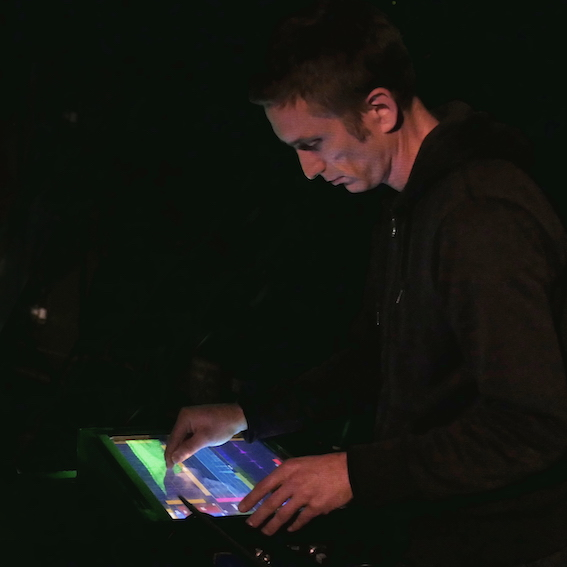
\includegraphics[width=\textwidth]{gfx/05_interfaces/xypre-v1_72dpi.jpg}
	\caption{xypre v1 inauguré durant une performance avec ONE}
	\label{fig:interface:xyprev1_jeu}
\end{figure}

Detecte tout ce qui est en contact (pas seulement les doigts mais aussi les objets) => permet de positionner des éléments de manière stable.

TOTO: insérer photo de la 1ère version (version concert)

\subsubsection{deuxième version}

%-------------------------- Figure : xypre ----------------------------------
\begin{figure}[!htbp]
	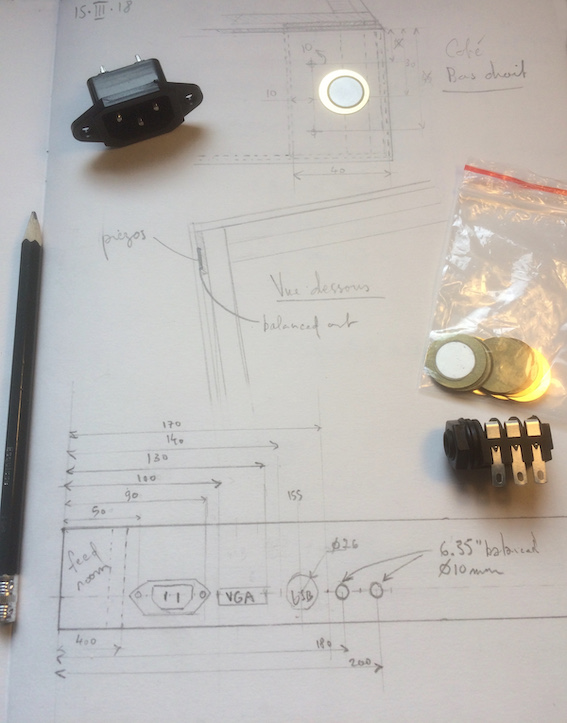
\includegraphics[width=\textwidth]{gfx/05_interfaces/Xypre_plan01_72dpi.jpg}
	\caption{xypre - plans de conception}
	\label{fig:interface:xypre_plans}
\end{figure}

%-------------------------- Figure : xypre ----------------------------------
\begin{figure}[!htbp]
	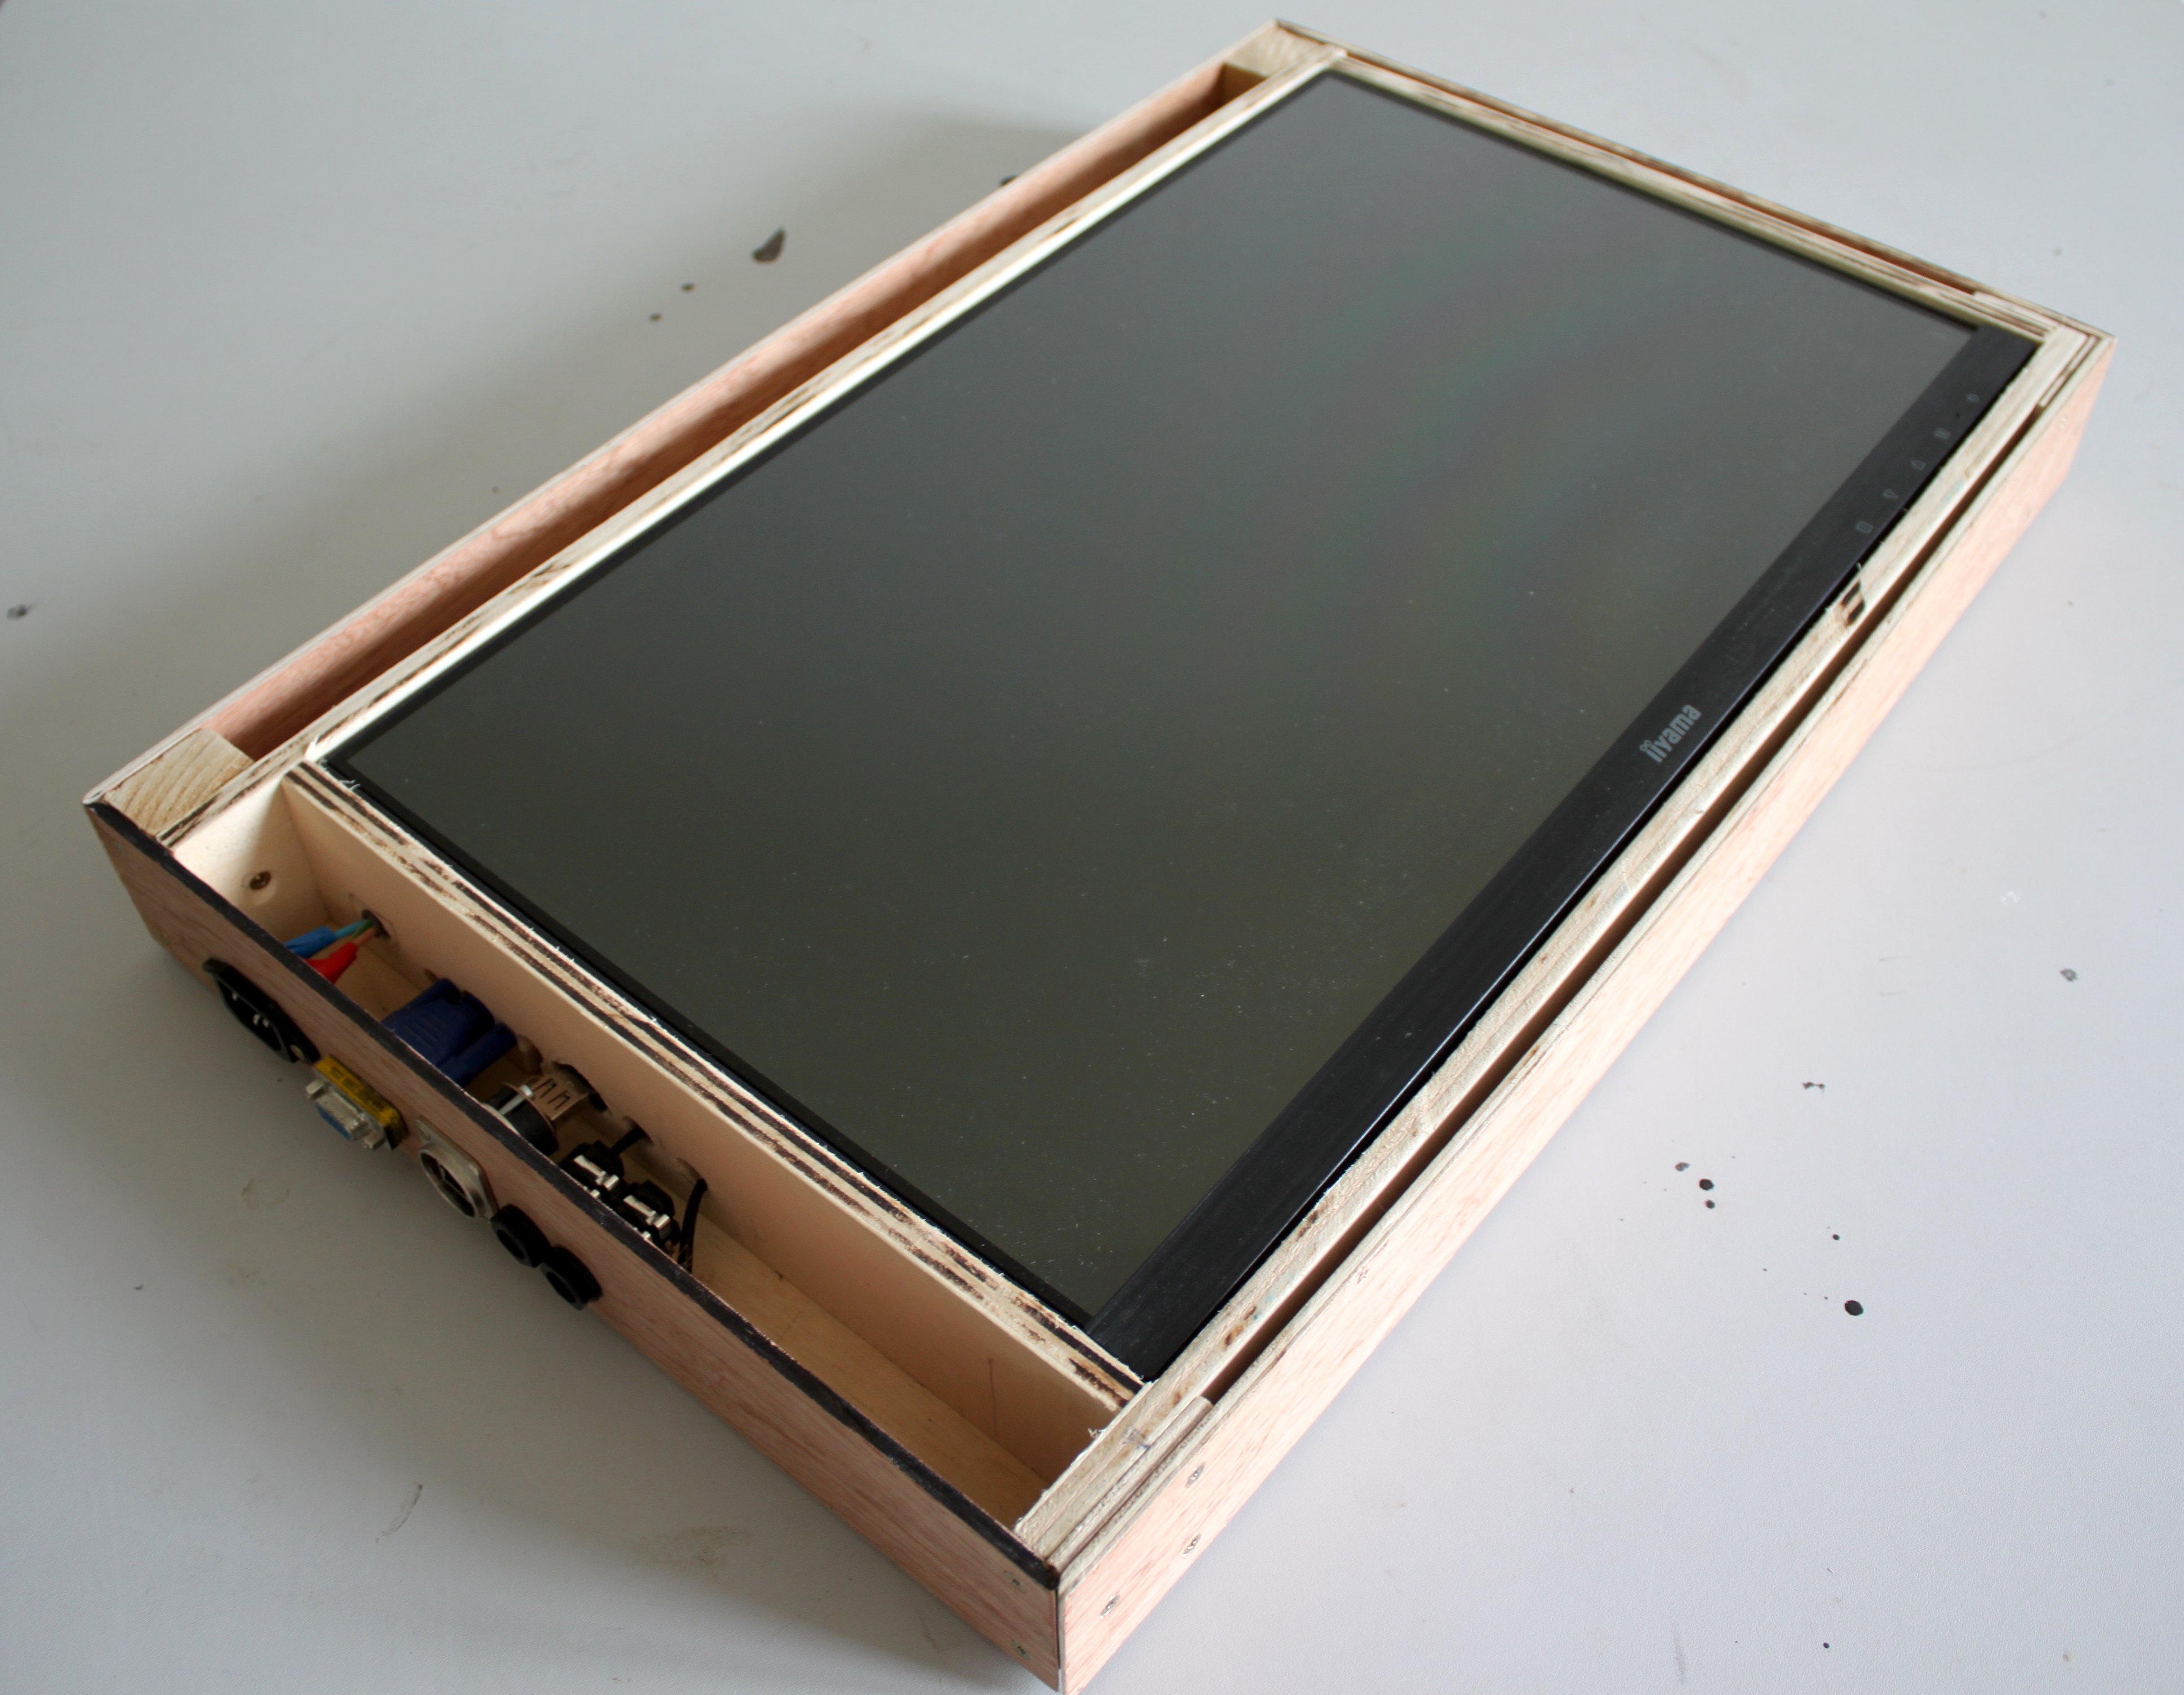
\includegraphics[width=\textwidth]{gfx/05_interfaces/xypre_overview_unplugged.jpg}
	\caption{xypre - vue d'ensemble, débranchée}
	\label{fig:interface:xypre}
\end{figure}

Ecran multitouch capacitif : détecte les doigts uniquement, pas les objets => motivation pour développer des objets positionnables de manière statique dans mp.TUI

Besoin d'un driver payant pour récupérer le TUIO.

Perte de la pression comme paramètre expressif :\\
intégration de capteur de pression (FSR) et de distance (IR)\\
Utilisation d'un Bela pour une latence très faible du son et un instrument autonome (needs raspberry for the display)\\
Possible extension par l'ordinateur.


%%%%%%%%%%%%%%%%%%%%%%%%%%%%%%%%%%%%%%%%%
\section{Conclusion}
\label{sec:interfaces:conclusion}


\section*{extra material}



%%%%%%%%%%%%%%

\iquote{Though there is a huge range of performer decision, history, and knowledge that will determine their exact method of playing (as established by Jorda [12]), the physical design of the DMI impacts this gesture repertoire by presenting certain affordances.} \cite{bin_hands_2017}

